\section{Конструкторский раздел}

% NOTE:
% В конструкторском разделе описывается разрабатываемый метод
% В случае если в бакалаврском проекте разрабатывается новый метод или алгоритм, необходимо подробно изложить их суть, привести все необходимые для их реализации математические выкладки, обосновать последовательность этапов выполнения
% При этом для каждого этапа следует выделить необходимые исходные данные и получаемые результаты
% Для описания метода или алгоритма - Схема алгоритма
% В конце описания разработанного алгоритма должны быть приведены выбранные способы тестирования и сами тесты
% Перед формированием тестовых наборов данных целесообразно указать выделенные классы эквивалентности
% (тут же могут быть приведены выкладки по теоретическим рассчетам требуемой памяти и эффективности алгоритма; эти результаты могут быть использованы для обоснования правильности выбора метода из уже имеющихся альтернативных вариантов)
% Также должно быть приведено описание структуры разрабатываемого ПО, оно включает в себя:
% - описание общей структуры - определение основных частей (компонентов) и их взаимосвязей по управлению и по данным
% - декомпозицию компонентов и построение структурных иерархий
% - проектирование компонентов
% Для графического представления такого описания (если есть необходимость), следует использовать IDEF0 с декомпозицией исходной задачи на несколько уровней

% Рек. Объем 25-30 страниц

\subsection{Требования и ограничения метода}

% Разработать метод выделения ... строке
% Изложить особенности предложенного метода

\subsection{Описание разрабатываемого метода}

% При этом для каждого этапа следует выделить необходимые исходные данные и получаемые результаты

% Сформулировать и описать ключевые шаги метода в виде схем алгоритмов

% Разработать алгоритм, реализующий данный метод

\subsection{Тестирование и классы эквивалентности}

\subsection{Структура разрабатываемого программного обеспечения}

\subsection*{Вывод}

% Основные этапы метода представлены на IDEF0-диаграмме первого уровня (см. Рисунок \ref{fig:a1}).
%
% \begin{figure}[H]
% 	\centering
% 	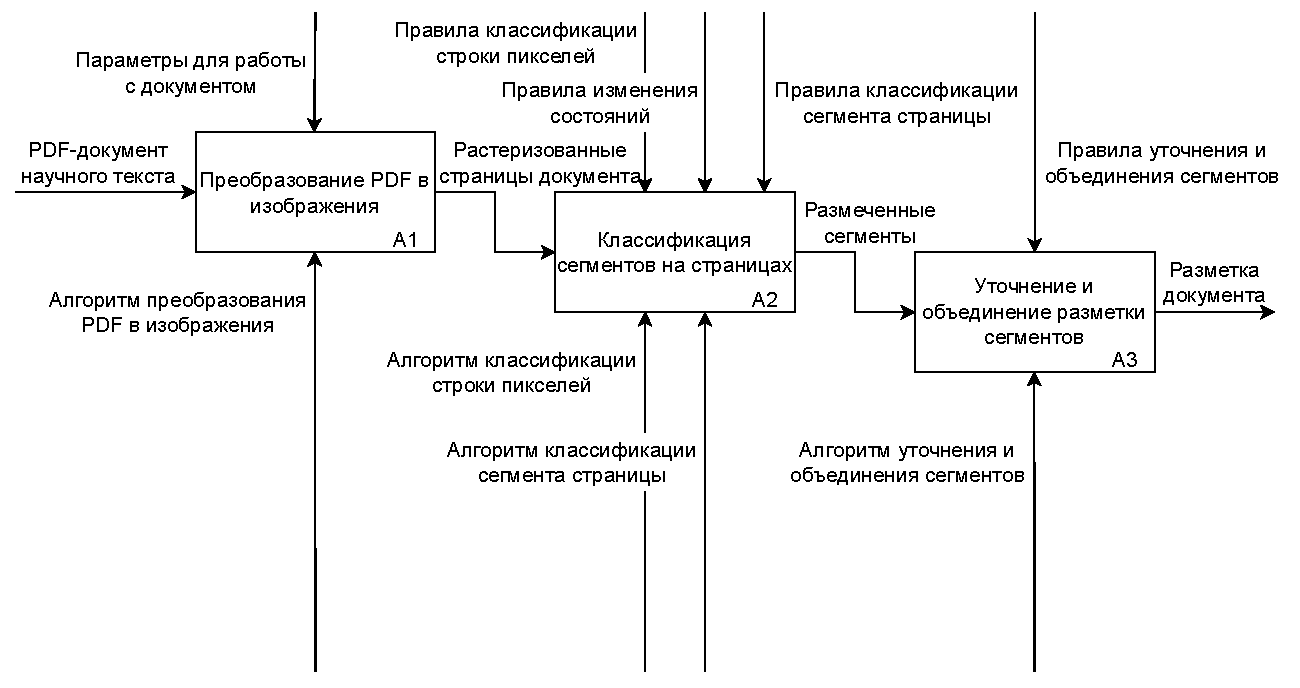
\includegraphics[width=\textwidth]{diag/a1-big.pdf}
% 	\caption{IDEF0-диаграмма метода выделения составных частей научного текста на основе анализа распределения пикселей в сканирующей строке}
% 	\label{fig:a1}
% \end{figure}
